% !TEX program = xelatex
% -------------------------------------------------------------
%  Clean CV template — Letter size (8.5 × 11 in)
%  Compile with **XeLaTeX**
% -------------------------------------------------------------

\documentclass[10pt,letterpaper]{article}

% ---------- ENCODING / FONTS ------------------------------------
\usepackage{fontspec}
\IfFontExistsTF{Roboto}
  {\setmainfont{Roboto}}
  {\setmainfont{Helvetica Neue}}

% ---------- GEOMETRY --------------------------------------------
\usepackage[
  letterpaper,
  left=0.55in,
  right=0.55in,
  top=0.8in,
  bottom=0.8in
]{geometry}

% ---------- COLOURS & GRAPHICS ----------------------------------
\usepackage[dvipsnames,svgnames,x11names]{xcolor}
\definecolor{primary}{HTML}{004A99}
\definecolor{accent}{HTML}{E6F4FF}

\usepackage{graphicx}
\usepackage{tikz}
\usetikzlibrary{calc}

% ---------- LAYOUT HELPERS --------------------------------------
\usepackage{paracol}
\columnratio{0.32}
\setlength{\columnsep}{0.25in}

\usepackage[most]{tcolorbox}
\tcbset{colback=accent,colframe=accent,boxrule=0pt,sharp corners}

\usepackage{enumitem}
\setlist[itemize]{noitemsep,topsep=0pt,leftmargin=*}

% ---------- HEADING STYLES --------------------------------------
\usepackage{sectsty}
\allsectionsfont{\color{primary}\bfseries\uppercase}
\subsectionfont{\color{primary}\bfseries}
\renewcommand{\thesection}{}

% ---------- UTILITIES -------------------------------------------
\newcommand{\cvName}[1]{\vspace*{0.3in}\textbf{\LARGE #1}}
\newcommand{\cvHeadline}[1]{\par\smallskip\textit{#1}}
\newcommand{\cvHr}{\vspace{0.5\baselineskip}\hrule height 1pt\color{primary}\vspace{0.7\baselineskip}}

%=================================================================
%                DOCUMENT
%=================================================================
\begin{document}

\begin{paracol}{2}

% -------- LEFT SIDEBAR ------------------------------------------
\begin{leftcolumn}
\begin{center}
\begin{tikzpicture}
  \node[draw=primary,line width=1pt,circle,minimum width=1.6in,minimum height=1.6in,inner sep=0pt]  (photo) {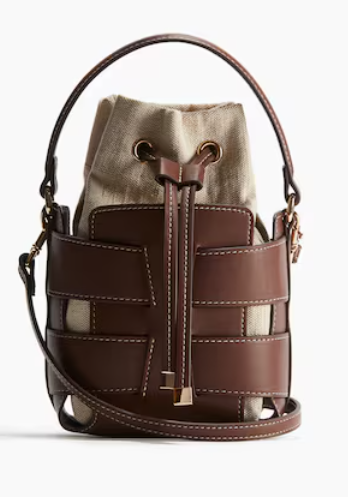
\includegraphics[width=1.6in,height=1.6in]{ed32bb11804f403c8c003ebad923a246.png}};
\end{tikzpicture}
\end{center}

\vspace{0.6in}

\cvName{Pape Saliou FALL}
\cvHeadline{Data Scientist}

\cvHr

\section*{Contact Information}
0753481453\\
papesalioufall2@gmail.com\\
Paris, Île-de-France, France

\cvHr

\section*{Languages}
Français (natif)\\
Anglais (courant)

\cvHr

\section*{Key Skills}
\begin{itemize}
  \item Python, R, SQL
  \item Pandas, NumPy, scikit-learn
  \item TensorFlow, PyTorch, Deep Learning
  \item Data Visualization (Plotly, Power BI)
  \item Spark, Docker, Git, MLOps
  \item AWS (S3, SageMaker), GCP (BigQuery)
\end{itemize}

\cvHr

\section*{Hobbies}
Randonnée, échecs, photographie urbaine

\end{leftcolumn}

% -------- MAIN COLUMN ------------------------------------------
\begin{rightcolumn}

\section*{Professional Summary}
Data Scientist avec une solide formation universitaire et une expérience pratique dans la conception de modèles de machine learning, l’analyse exploratoire de données et la mise en production de solutions data-driven. Passionné par la transformation des données brutes en informations stratégiques, je maîtrise Python, SQL, les bibliothèques ML (scikit-learn, TensorFlow, PyTorch), ainsi que les environnements cloud (AWS, GCP). Orienté résultats, j’apprécie le travail en équipe agile et la communication de la valeur business via des visualisations claires et des rapports pertinents.

\vspace{1in}

\section*{Work Experience}

\begin{tcolorbox}
  \begin{minipage}[t]{0.48\linewidth}
    Sep 2022\\
    \textbf{Prepaya — Paris, France}\\
    \textit{Data Scientist}
    \begin{itemize}
      \item Développé et déployé des modèles de prévision de churn utilisant XGBoost, augmentant la précision de 15 \% par rapport à la solution précédente.
      \item Élaboré des pipelines ETL automatisés (Python, Airflow) pour collecter et nettoyer plus de 50 Go de données clients hebdomadaires.
      \item Créé des tableaux de bord interactifs sous Power BI permettant aux équipes marketing de suivre les KPI en temps réel.
      \item Implémenté des tests unitaires et une CI/CD via GitLab pour fiabiliser le cycle de vie des modèles.
      \item Collaboré avec les équipes produit et business pour traduire les besoins métier en spécifications techniques.
      \item Réalisé des analyses ad-hoc (SQL, Pandas) afin d’identifier des segments clients à haut potentiel.
      \item Assuré la documentation complète des modèles et des jeux de données, facilitant la maintenance et la reprise de projet.
    \end{itemize}
  \end{minipage}\hfill
  \begin{minipage}[t]{0.48\linewidth}
    \raggedleft
    Aug 2023
  \end{minipage}
\end{tcolorbox}

\vspace{0.9in}

\section*{Education}
\begin{tcolorbox}[colback=white,boxrule=1pt,colframe=primary]
  \begin{minipage}{0.47\linewidth}
    2022 – 2023\\
    \textbf{Sorbonne Université}\\
    Master 2 — Data Science
  \end{minipage}
\end{tcolorbox}

\section*{Certifications}
\begin{itemize}
  \item 02/2024 — TensorFlow Developer Certificate, Google
  \item 11/2023 — AWS Certified Machine Learning – Specialty, Amazon Web Services
\end{itemize}

\end{rightcolumn}

\end{paracol}

\end{document}